\paragraph{}
Nos ultimos anos o \textit{OpenSource} esta tendo uma crescente, após empresas como: Microsoft, Google, Facebook, começarem a disponibilizar alguns de seus \textit{softwares} utilizados internamente para a comunidade de \textit{software} livre.
Utilizando o GitHub, um dos maiores hubs de código e \textit{networking} de desenvolvedores do mundo, essas empresas conseguem disponibilizar seu \textit{software} em repositórios regido por uma licença, onde é descrito o que é exigido, permitido e probido com o \textit{software} em questão.

\paragraph{}
Ao pesquisar sobre licenças de \textit{software} livre é possível encontrar vários tipos para todos os casos, tudo depende do ponto em que o mantenedor do projeto quer chegar, seja eles, trabalhar em comunidade (MIT), estar preocupado com patentes (Apache) ou apenas compartilhar melhorias (GPLv2 ou GPLv3) \cite{choosealicense}.
A partir disso ja podemos ter uma noção de qual o caminho que um software consegue chegar de acordo com uma licença. Ja se sabe que isso não caba influenciando cem por cento, que o fato de ter alguma empresa grande por trás ja é um grande fator, porém há outros fatores que podemos analisar para poder chegar nesse ponto de popularidade como citado no trabalho do Borges, Hora e Valente \cite{borges2016understanding}.

\paragraph{}
Inspirados pelos botões de redes sociais modernas, os usuários do GitHub também podem estrelar um repositório, presumivelmente para manifestar interesse ou satisfação com o projeto hospedado\cite{gousios2014exploratory, gousios2015work}.
Por exemplo, os desenvolvedores podem separar sua própria cópia de um repositório, trabalhar e melhorar o código localmente e, em seguida, enviar uma solicitação \textit{pull} para integrar as mudanças no repositório principal\cite{borges2016understanding}. Gerando assim uma popularidade de alguns projetos, e tirando esse proveito de semelhanças com redes sociais fica mais fácil poder analisar o que é tendencia ou não, já que os indices de cada projeto ja estão definidos por alguns indices mostrados na Figura \ref{fig:github-linux}
\begin{figure}[h!]
    \centering
    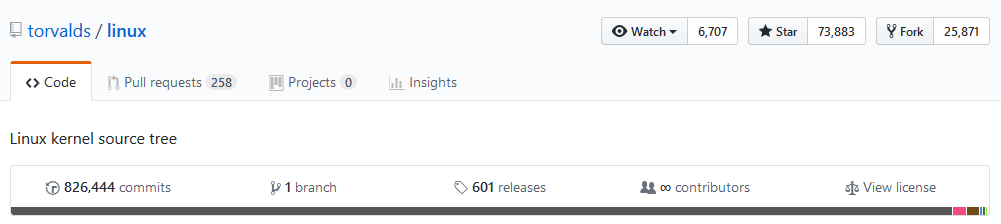
\includegraphics[width=\linewidth]{assets/images/github-linux.PNG}
    \caption{Exemplo de Repositório no Github (Kernel Linux)}
    \label{fig:github-linux}
\end{figure}

\paragraph{}
